% document type
\documentclass[twocolumn,final]{svjour3}
\smartqed  % flush right qed marks, e.g. at end of proof
% packages
%\usepackage{cite}
\usepackage[pdftex]{graphicx}
\usepackage{amsmath}			% Advanced math typesetting
\usepackage{algorithm}
\usepackage{algpseudocode}		% pseudocode support 
\usepackage[english]{babel}		
% Change hyphenation rules for the words where needed
\babelhyphenation[english]{al-go-rithms clus-te-red par-ti-tion-ing bi-par-ti-tion-ing sig-ni-fi-cant-ly sur-veil-lance ap-pro-ach-es re-gi-on over-view pipe-li-ne me-thod seg-men-ta-ti-on un-der-seg-men-ta-ti-on ov-er-seg-men-ta-ti-on per-forms strong-ly un-der spe-ci-fi-cal-ly Tas-ter Cham-paign re-gi-on im-ple-men-ted where-as}

\usepackage[hidelinks]{hyperref}% Add http links to your document
%\hypersetup{final}
\usepackage{enumitem}			% for the list
\usepackage{array}				% for tables
\usepackage{flushend}			% equal last columns length

\newcommand{\norm}[1]{\left\lVert #1 \right\rVert}
\newcolumntype{C}[1]{>{\centering\let\newline\\\arraybackslash\hspace{0pt}}m{#1}}

\begin{document}

\author{Stanislav Protasov \and A2}
% university and contact email
\institute{Russia, Innopolis, Innopolis University, \\\email{s.protasov@innopolis.ru}}
\title{Proximity graphs application to large scale classification}
% first author is here
\authorrunning{Protasov et al.}  
\maketitle{}					% Generates title


% tell about main problem and result. Better have 1-2 short sentences for each part
\begin{abstract}
% problem
Billion-scale datasets can be a big problem for building fast and compact classifiers.
% task
We are targeting fast and scalable data structures and algorithms that allow to build instance-based classifiers for multidimensional data.
% how we solve it
We propose two classifier approaches based on analysis of proximity graph, built upon large dataset.
% results
For both approached we gained interesting theoretical results. Greedy approach showed 10x average speedup for classification based compared to production library.
% application
...
\keywords{indexing \and classification \and graphs \and proximity graphs}
\end{abstract}

\section{Introduction}\label{sec:INTRO}

% here you start with discussion of a bigger problem, and go to the conclusion that the !!problem (not task)!! you are trying to solve is very important.

Text \cite{jia2014caffe}

% in the end you end up with a structure

The paper is organized as follows.
In section~\ref{sec:OVERVIEW} we discuss related works including contemporary approaches to ....
Section~\ref{sec:METHOD} is devoted to our proposed methodology for ....
In section~\ref{sec:METHODRESULTS} we present experimental results.
These results are then discussed in section~\ref{sec:DISCUSSION},
and conclusions are drawn in section~\ref{sec:CONCLUSION}.

\section{Relates works}\label{sec:OVERVIEW}

% start filling this section with the following templates:

In paper \cite{jia2014caffe} authors propose XXX. They are solving problem XXX using XXX. New idea of their work is XXX. Strong part of this work is XXX. Weak part of this work is XXX.


% also if possible contribute general comments here. Examples are:

%% - all the works are using different datasets, that's why it is impossible to compare.
%% - all works use different quality metrics, which make them incomparable.
%% - most of works lacks necessary information for reproduction
%% - all solutions tend to use technology X
\section{Methodology}\label{sec:METHOD}
%% this part will hold all necessary data for our method reproduction
%% we explicitly explain what decision were made, what libraries and hardware were used

%% below you see some examples of how to embed images and tables


%% how to embed image for 2 columns
\begin{figure*}[ht]
	\normalsize
    \centering
    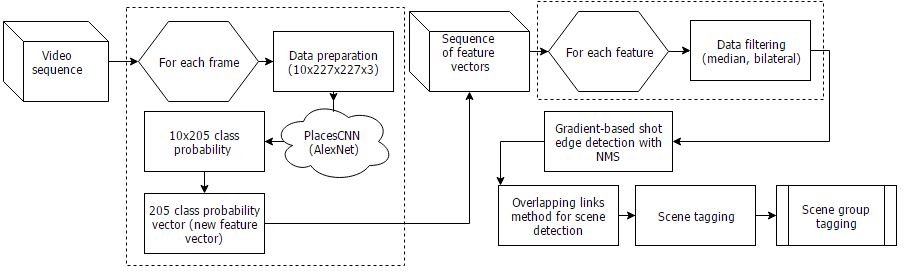
\includegraphics[width=6.3in]{images/Fig1.png}
    \caption{The title}
    \label{fig:workflow}
\end{figure*}

An overview of the proposed approach is shown in figure \ref{fig:workflow}.

%% how to embed 1-column image
\begin{figure}
    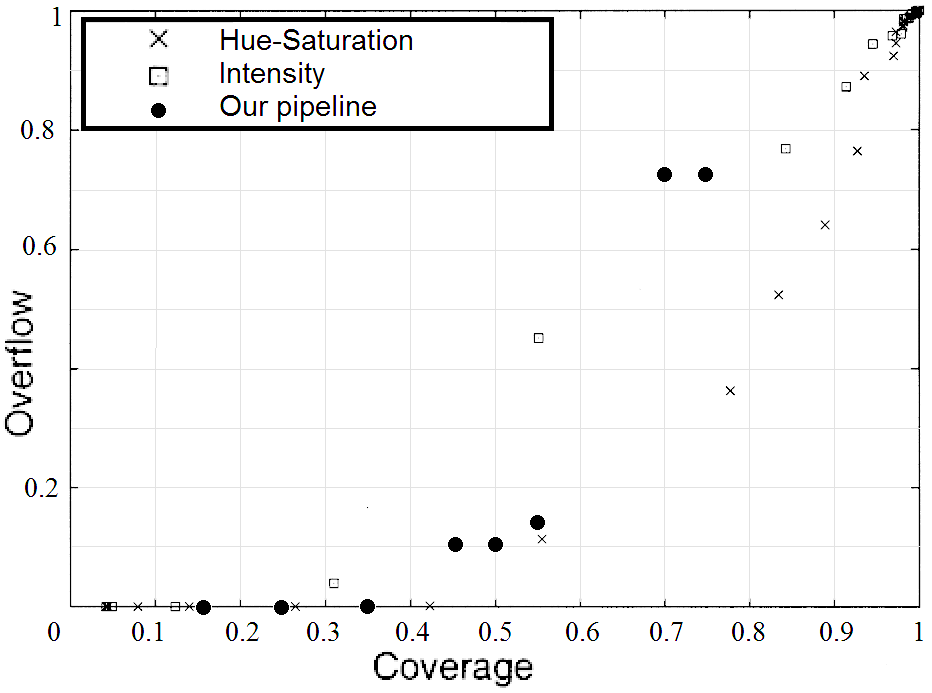
\includegraphics[width=3.3in]{images/Fig2.png}
    \caption{Comparison of coverage and overflow metrics values for our pipeline with original paper}
    \label{fig:cov-over}
\end{figure}

This is how we refer this image \ref{fig:cov-over}.


%% how to embed table
\begin{table}
\caption{Oversegmentation with different filters for top achieved accuracies for 30fps dataset}
\label{tb:oversegment}
\centering
\begin{tabular}{ | c | p{16mm} | p{16mm} | c | }
\hline
\textbf{Filter} & \textbf{Param.} & \textbf{Edge det. \newline accuracy} & \textbf{Oversegm.} \\
\hline
No filter & -- & 0.929 & 10.571 \\
\hline
Median & $W=3$ & \textbf{0.982} & 13.5 \\
\hline
Median & $W=5$ & 0.964 & \textbf{8.75} \\
\hline
Bilateral & ${\sigma}_{g}=1,\newline {\sigma}_{f}=0.1$ & 0.964 & 12.5 \\
\hline
Bilateral & ${\sigma}_{g}=1,\newline {\sigma}_{f}=0.3$ & 0.964 & 13.732 \\
\hline
\end{tabular}
\end{table}

This is how we refer tables: ~\ref{tb:oversegment}.
\section{Results}\label{sec:METHODRESULTS}

%% here we will discuss results of our work. Consider and compare quality metrics, show interesting finding. E.g.g

Among xxx we found a strong positive correlation xxx. That means the xxx.
This can be explained by xxx.
\section{Discussion}\label{sec:DISCUSSION}

%% discussion is meant for interpretation of results. Here we can discuss where we succeeded more, over-perform someone's work or even fail.
%% You can start your section with something like this.
%% e.g.
We will discuss the results of our work from two points of view.
Firstly we analyze the existing and proposed metrics.
We discuss how expressive the quality metrics are.
The second part presents our findings: best algorithm parameters, performance and improvements.
\section{Conclusion}\label{sec:CONCLUSION}
%% Conclusion is an extended version of annotation. It usually expands some major results of the work with numbers. And also it adds some place for future work. E.g.
In future we plan to xxx. We are also going to xxx.

% bibliography settings
\bibliographystyle{spmpsci}
% link to bibtex file
\bibliography{links}
\end{document}